\textbf{¿Cuál es el perímetro del paralelogramo de la figura \ref{fig:peri_paralelogramo_01}?}\\
\emph{Considera que cada cuadro mide 1 unidad de longitud.}

\begin{figure}[H]
    \centering
    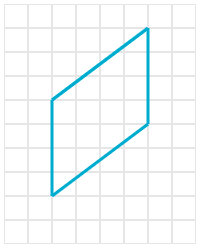
\includegraphics[width=0.25\linewidth]{../images/peri_paralelogramo_01.png}
    \caption{}
    \label{fig:peri_paralelogramo_01}
\end{figure}

\begin{solutionbox}{14cm}
    \begin{minipage}{0.4\textwidth}
        \begin{multicols}{2}
            \begin{figure}[H]
                \centering
                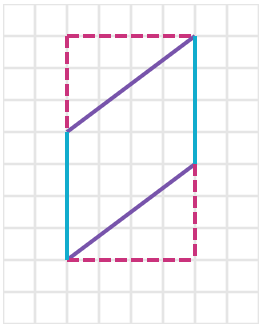
\includegraphics[width=0.9\linewidth]{../images/peri_paralelogramo_01a.png}
                \caption{}
                \label{fig:peri_paralelogramo_01a}
            \end{figure}
            \begin{figure}[H]
                \centering
                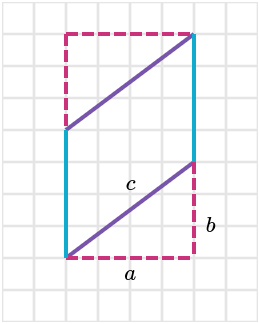
\includegraphics[width=0.9\linewidth]{../images/peri_paralelogramo_01b.png}
                \caption{}
                \label{fig:peri_paralelogramo_01b}
            \end{figure}
        \end{multicols}
        \begin{multicols}{2}
            \begin{figure}[H]
                \centering
                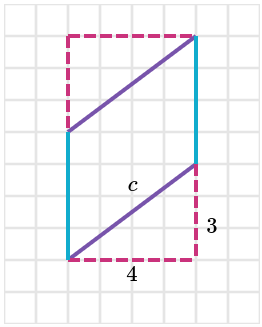
\includegraphics[width=0.9\linewidth]{../images/peri_paralelogramo_01c.png}
                \caption{}
                \label{fig:peri_paralelogramo_01c}
            \end{figure}
            \begin{figure}[H]
                \centering
                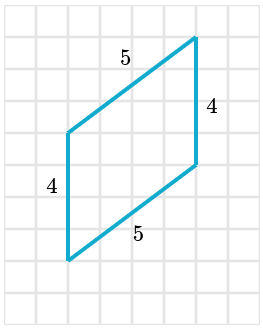
\includegraphics[width=0.9\linewidth]{../images/peri_paralelogramo_01d.png}
                \caption{}
                \label{fig:peri_paralelogramo_01d}
            \end{figure}
        \end{multicols}
    \end{minipage}\hfill
    \begin{minipage}{0.5\textwidth}
        El perímetro es la distancia alrededor de una figura.
        Cada recta diagonal es la hipotenusa de un triángulo rectángulo (ver Figura \ref{fig:peri_paralelogramo_01a}).
        Podemos utilizar el teorema de Pitágoras para encontrar un lado faltante.
        La ecuación del teorema de Pitágoras es:
        \[c^2=a^2+b^2\]
        donde $a$ y $b$ son las longitudes de los catetos, y $c$ es la longitud de la hipotenusa.
        Etiquetemos la Figura del problema con $a$, $b$ y $c$ (ver Figura \ref{fig:peri_paralelogramo_01b}).
        Podemos contar los cuadrados para encontrar las longitudes de $a$ y $b$, y luego sustituir esos valores en el teorema de Pitágoras (ver Figura \ref{fig:peri_paralelogramo_01c}).
        \begin{align*}
            a^2+b^2  =c^2 & \text{\quad El teorema de Pitágoras}                          \\
            4^2+3^2  =c^2 & \text{\quad Sustituye las longitudes}                         \\
            16 +9 =c^2    & \text{\quad Evalua los cuadrados conocidos}                   \\
            25=c^2        & \text{\quad Sumando }                                         \\
            5=c           & \text{\quad Calculando la raíz en ambos lados de la ecuación} \\
        \end{align*}
        Ahora que conocemos la longitud de la diagonal, podemos encontrar la longitud de los dos lados faltantes para calcular el perímetro.
        Como los lados faltantes son rectas verticales u horizontales, podemos contar los cuadrados para obtener sus longitudes. (ver Figura \ref{fig:peri_paralelogramo_01d}).
        \[5+5+4+4=18\]
        El perímetro del paralelogramo es 418 unidades.
    \end{minipage}
\end{solutionbox}
